\section{Valutazione delle Prestazioni}
Vista la particolare architettura, uno dei problemi che potrebbero scaturire è quello di eventuali "colli di
bottiglia", ossia rallentamenti con l'aumentare del numero di attori del modello. Pertanto, è stato ritenuto opportuno
effettuare una rilevazione dei tempi di scambio dei messaggi per fare considerazioni sulle prestazioni del paradigma
applicato al pattern \textbf{MVC}.

\begin{figure}[H]
    \centering
    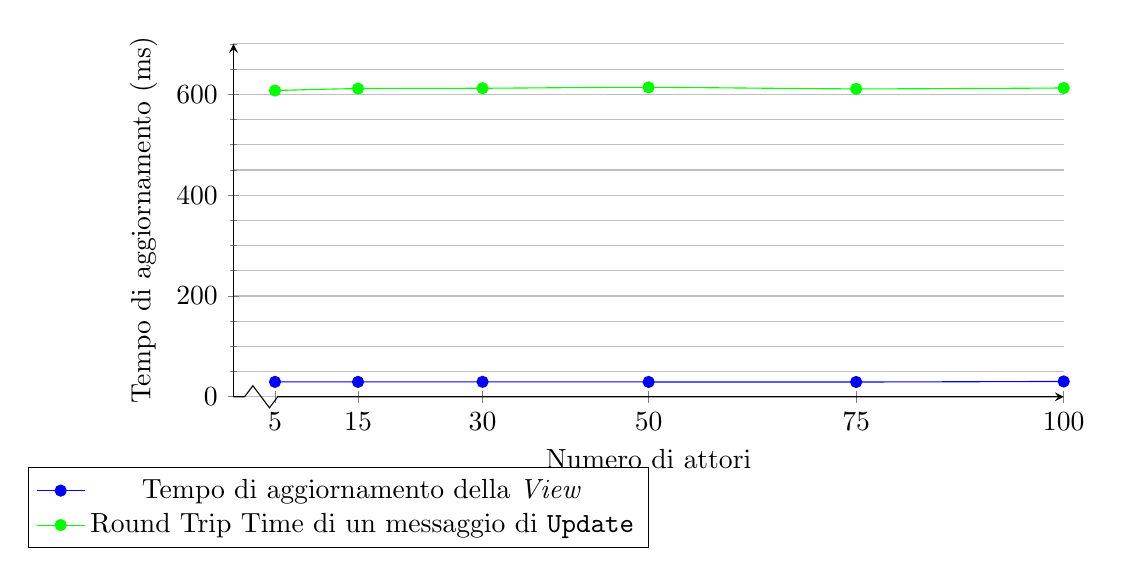
\begin{tikzpicture}
        \begin{axis}[
        xmin=0, xmax=100,
        ymin=0, ymax=700,
        xtick={5,15,30,50,75,100},
        minor ytick={0,50,...,700},
        axis x line=bottom,
        axis y line=left,
        axis x discontinuity=crunch,
        ymajorgrids=true,
        yminorgrids=true,
        xlabel={Numero di attori}, ylabel={Tempo di aggiornamento (ms)}, title={},
        axis on top=true, clip=false,  width=\textwidth, height=.5\textwidth,
        legend style={
            at={(0,0)},
            anchor=north east,
            at={(axis description cs:0.5,-0.2)}}
        ]
        \addplot [mark=*, mark options={solid}, smooth, color=blue] coordinates {
            (5, 29.5)
            (15, 29.5)
            (30, 29.6)
            (50, 29.4)
            (75, 29.3)
            (100, 30.4)
        };
        \addplot [mark=*, mark options={solid}, smooth, color=green] coordinates {
            (5, 607.5)
            (15, 611.4)
            (30, 612.1)
            (50, 613.9)
            (75, 610.9)
            (100, 612.6)
        };
        \legend{Tempo di aggiornamento della \textit{View}, Round Trip Time di un messaggio di \texttt{Update}};
        \end{axis}
    \end{tikzpicture}
    \caption{Rilevazione dei tempi di scambio messaggi del \texttt{GameLoop}
    \label{fig:performance-evaluation}}
\end{figure}

Per ottenere i risultati mostrati in figura \ref{fig:performance-evaluation}, sono state effettuate diverse misurazioni
e ne è stata calcolata la media. In particolare, vengono mostrati i tempi di aggiornamento della \texttt{View} e il
tempo che impiega un messaggio di \texttt{Update} a partire dal \texttt{GameLoop}, aggiornare il \texttt{Model} e
tornare al mittente. Come ci si aspettava, i valori misurati non variano notevolmente con l'aumentare del numero degli
attori: la frequenza d'aggiornamento della \texttt{View} si mantiene attorno ai 30 millisecondi, mentre il
\textit{round-trip time} degli \texttt{Update} attorno ai 600 millisecondi. Si conclude che il paradigma ad attori
non comporta problemi di scalabilità sul numero di entità nel modello.